\chapter{Implementation}
\label{implementation}
\section{Introduction}
Following the design process, the two elements were designed separately and then integrated with Infandango. This step required understanding of how the Infandango system works, specifically how it renders webpages. The completed system gives a visual display for the predicted score retrieved from the model.

\section{Language and Tools}
Two languages are immediate possibilities for implementation: Java\cite{java_site} and Python\cite{python_site}. Java because I had the most experience with it and some parts of Infandango are written in Java. Most of Infandango was, however, written in Python with which I also had experience. Due to the emphasis the project has on machine learning, R\cite{r_site} was another approriate language. 
The final decision was to use Python with scikit-learn\cite{scikit_site} and pybrain\cite{pybrain2010jmlr} libraries: this provides the simplest integration with Infandango (since the parts with which this will need to be integrated are written in Python) and the libraries provide a variety of machine learning methods.

\section{Visual Design}
The final design is relatively simple and since the system is web based web technologies like Javascript and CSS were considered. The choice between implementation strategies was based on the ease of integration with Infandango: although Infandango does already use Javascript like the Scriptaculous library\cite{scriptaculous_site}, CSS is more heavily used. For example, the lab exercise page Infandango displays a single score for an exercise with a background colour determined by the score (red for a bad score, green for a good score). pure CSS is used here where Javascript could also have been, and so a similar CSS based approach was used for the visualisation.

\section{Prediction Model}
The majority of the implementation for the model has already been performed when choosing the appropriate model: loading data, parsing data, training the model and performing a prediction. The final remaining step is allowing Infandango access to the model, a problem for which two solutions were immediately considered.

The first solution is to load the data and train the model when Infandango first starts. This object would then passed around to the appropriate place, staying in memory and being used whenever it is needed. Some problems with this model are:

\begin{enumerate}
\item it makes changing the model during runtime more or less impossible without restarting Infandango
\item the data used for training would also need to be stored somewhere, which could require a separate database running alongside the active database \item it could potentially cause some coupling between the code used for training the model and the Infandango startup procedure, making future adaptations more difficult
\end{enumerate}

The second solution is training the model before hand and storing/loading this model to be used when necessary. A problem with this approach is that loading the model must occur during runtime which could potentially slow the loading speed of the web page. However, this approach does overcome some of the problem of the previous approach: 

\begin{enumerate}
\item the model can be changed easily, providing it uses the same loading interface
\item only the model needs to be stored, not all the data used for training
\item any model and training procedure can be used, as long as the same call can be made to make a prediction.
\end{enumerate}

The final implementation uses the training procedures discussed in chapter \ref{machinelearning} to train the model and serialises it using the standard python module, pickle\cite{pythonpickle_site}.

\section{System Integration}
Infandango uses Django to generate the web pages. Django uses python to generate webpages and thus allows dynamic content to be inserted into the webpage. Each page has a method which generates this content which can be used specifically for that page. Since the progress bar is attaching to the sidebar - an item which appears on every page - then manually adding the prediction code to every page would take time, would be very difficult to change and is generally undesirable. Instead, Django offers "Context Processors" which is a way of hooking methods into the call that loads every page, allowing this content to be used by any page without telling every page explicitly. This also makes changing/removing the functionality much simpler. 

\section{Technical Issues}

\subsection{Neural Network Hidden Layers}
Although Pybrain provides many different types of hidden layers only two were used: Sigmoid and Tanh. All attempts with other layers would lead to an error due to an overflow occuring, perhaps caused by the amount of data used. These errors may not happen for Sigmoid and Tanh layers as they are squashing functions.

\subsection{Slow Neural Networks}
The Pybrain library was used due to it being written in Python and its ease of use. However, a factor not fully considered at first was the speed. Although the speed is not a problem when performing a prediction, however it becomes an impediment when performing optimisation and cross-fold validation. In an effort to mitigate this problem, the arac library\cite{arac_site} was used, which is used in conjunction with Pybrain to provide fast implementations of the neural networks provided by Pybrain. Due to the alpha state of the project some additional time was needed after installation in order to debug the library, but a working solution was found which on average reduced neural network training time by 50%.

\section{Conclusion}
Using the Django context processor functionality a function is hooked into every web page request. This function de-serialises the trained model and uses it to provide a prediction based on previous exercise submissions. This prediction is used to determine the colours which will be displayed in each box and this is facilitated through Django. Figure \ref{fig:contextprocessor} shows the control flow of this process.

\begin{figure}[h!]
\centering
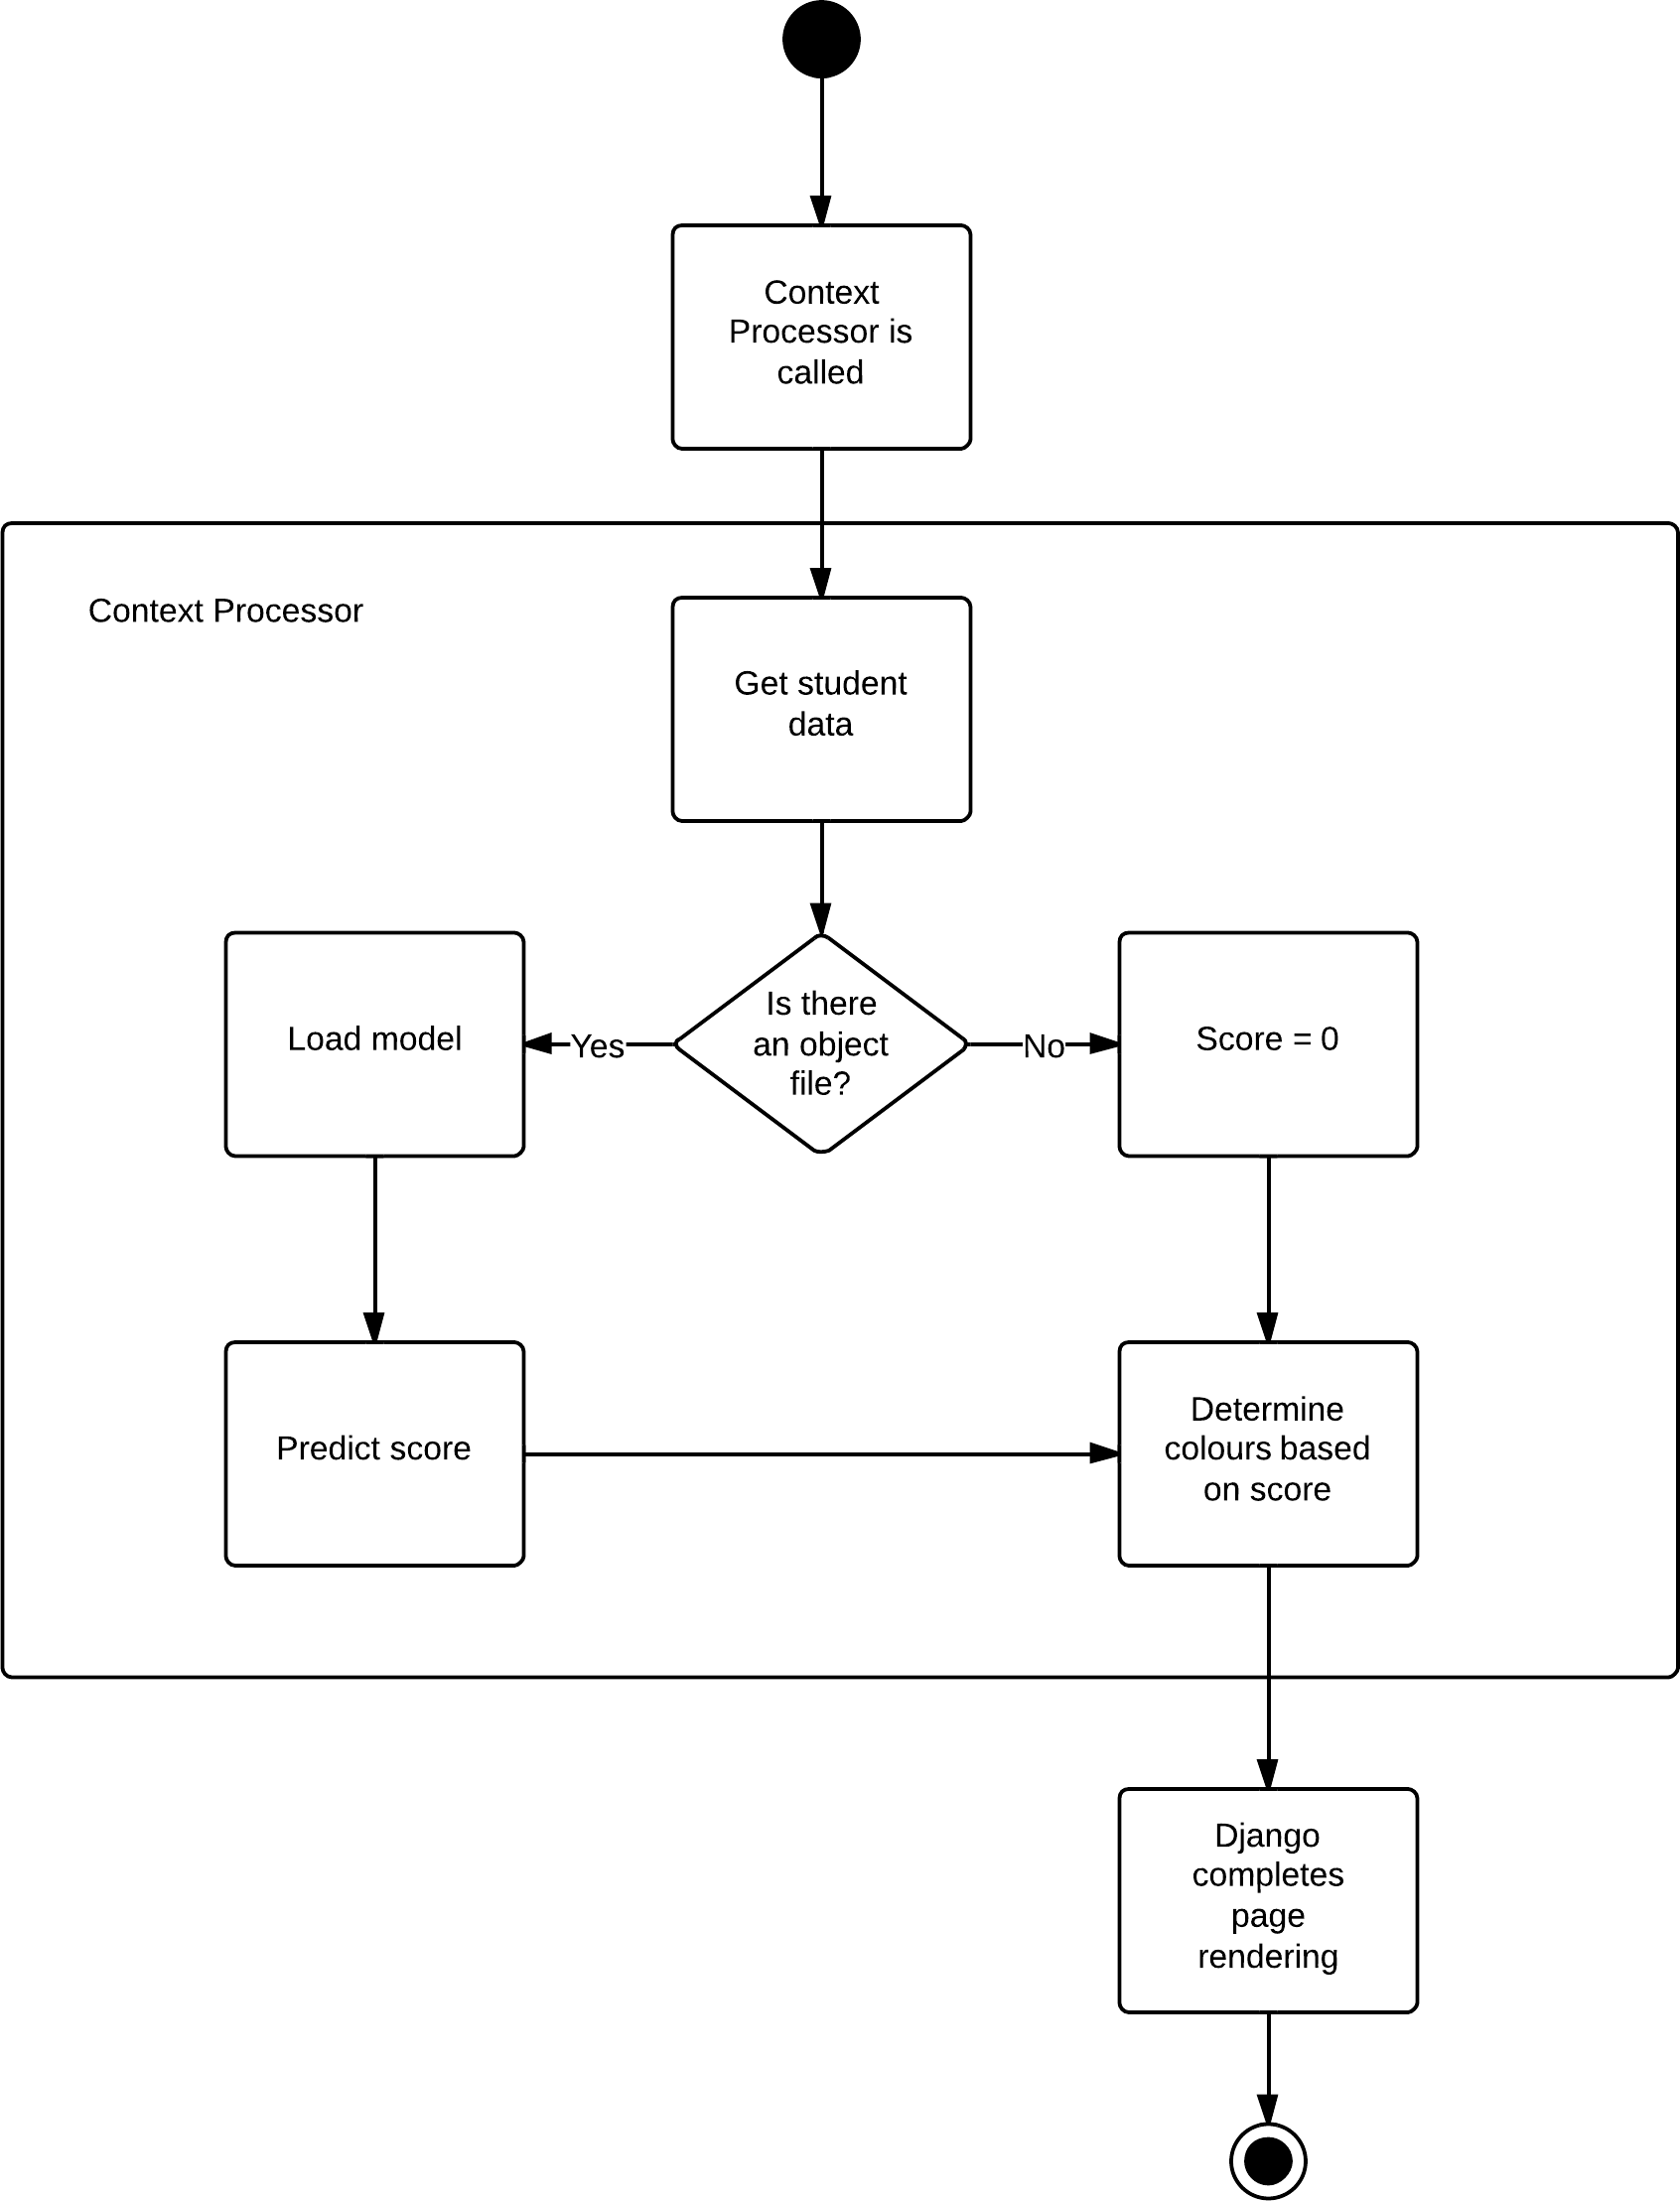
\includegraphics[width=0.8\textwidth]{images/contextprocessor.png}
\caption{A flowchart of the context processor function and how it interacts with Django}
\label{fig:contextprocessor}
\end{figure}
